%%%%%%%%%%%%%%%%%%%%%%%%%%%%%%%%%%%%%%%%%%%%%%%%%%%%%%%%%%%%%%%%%%%%%%%
% Factor Trajectory Card - Institutional_Momentum_Score_20D
% Complete Factor Evolution History
%%%%%%%%%%%%%%%%%%%%%%%%%%%%%%%%%%%%%%%%%%%%%%%%%%%%%%%%%%%%%%%%%%%%%%%

\documentclass[11pt,a4paper]{article}
\usepackage{geometry}
\usepackage{xcolor}
\usepackage{tikz}
\usepackage{tcolorbox}
\usepackage{booktabs}
\usepackage{amsmath}
\usepackage{amssymb}
\usepackage{fontawesome5}
\usepackage{hyperref}
\usepackage{listings}
\usepackage{multirow}
\usepackage{graphicx}

\geometry{margin=2cm}

% Color definitions
\definecolor{headerblue}{RGB}{41, 128, 185}
\definecolor{metricgreen}{RGB}{39, 174, 96}
\definecolor{alertred}{RGB}{192, 57, 43}
\definecolor{warningyellow}{RGB}{243, 156, 18}
\definecolor{lightgray}{RGB}{245, 245, 245}
\definecolor{darkgray}{RGB}{52, 73, 94}
\definecolor{mutationpurple}{RGB}{142, 68, 173}
\definecolor{crossoverblue}{RGB}{52, 152, 219}

% tcolorbox styles
\tcbuselibrary{skins,breakable}

\newtcolorbox{factorbox}[2][]{
  colback=lightgray,
  colframe=headerblue,
  fonttitle=\bfseries\large,
  title=#2,
  arc=3mm,
  boxrule=1pt,
  #1
}

\newtcolorbox{hypothesisbox}[1][]{
  colback=blue!5,
  colframe=headerblue!70,
  fonttitle=\bfseries,
  title={\faLightbulb\ Hypothesis},
  arc=2mm,
  boxrule=0.5pt,
  #1
}

\newtcolorbox{metricsbox}[1][]{
  colback=green!5,
  colframe=metricgreen,
  fonttitle=\bfseries,
  title={\faChartLine\ Backtest Metrics},
  arc=2mm,
  boxrule=0.5pt,
  #1
}

\newtcolorbox{feedbackbox}[1][]{
  colback=yellow!5,
  colframe=warningyellow,
  fonttitle=\bfseries,
  title={\faComments\ Feedback \& Evaluation},
  arc=2mm,
  boxrule=0.5pt,
  #1
}

\newtcolorbox{evolutionbox}[1][]{
  colback=purple!5,
  colframe=mutationpurple,
  fonttitle=\bfseries,
  title={\faDna\ Evolution Information},
  arc=2mm,
  boxrule=0.5pt,
  #1
}

\begin{document}

%%%%%%%%%%%%%%%%%%%%%%%%%%%%%%%%%%%%%%%%%%%%%%%%%%%%%%%%%%%%%%%%%%%%%%%
% Title Section
%%%%%%%%%%%%%%%%%%%%%%%%%%%%%%%%%%%%%%%%%%%%%%%%%%%%%%%%%%%%%%%%%%%%%%%
\begin{center}
{\LARGE\bfseries\color{headerblue} Factor Trajectory Card}\\[0.5cm]
\rule{\textwidth}{1pt}
\end{center}

%%%%%%%%%%%%%%%%%%%%%%%%%%%%%%%%%%%%%%%%%%%%%%%%%%%%%%%%%%%%%%%%%%%%%%%
% Basic Information
%%%%%%%%%%%%%%%%%%%%%%%%%%%%%%%%%%%%%%%%%%%%%%%%%%%%%%%%%%%%%%%%%%%%%%%
\begin{factorbox}{\faTag\ Institutional\_Momentum\_Score\_20D}

\begin{tabular}{@{}ll@{}}
\textbf{Factor ID:} & \texttt{c57cace576a95356} \\
\textbf{Trajectory ID:} & \texttt{df5a496878f4} \\
\textbf{Experiment ID:} & \texttt{2026-01-21\_16-23-59-525038} \\
\textbf{Created At:} & 2026-01-22 17:23:36 \\
\textbf{Evolution Round:} & Round 8 \\
\textbf{Evolution Phase:} & \colorbox{crossoverblue!20}{\textcolor{crossoverblue}{\textbf{Crossover}}} \\
\textbf{Direction ID:} & 6 \\
\end{tabular}

\vspace{0.3cm}

\textbf{Factor Expression:}
\begin{tcolorbox}[colback=darkgray!5, colframe=darkgray, boxrule=0.3pt, arc=1mm]
\small\ttfamily
RANK(TS\_CORR(DELTA(\$close, 1)/\$close, DELTA(\$volume, 1)/\$volume, 20) * TS\_MEAN((\$close - \$open)/\$close, 5))
\end{tcolorbox}

\textbf{Mathematical Formulation:}
\[
\text{IMS}_{20D} = \text{RANK}\left(\text{TS\_CORR}\left(\frac{\Delta \text{close}}{\text{close}}, \frac{\Delta \text{volume}}{\text{volume}}, 20\right) \times \text{TS\_MEAN}\left(\frac{\text{close} - \text{open}}{\text{close}}, 5\right)\right)
\]

\textbf{Factor Description:}\\
\small
This factor measures the correlation between price returns and volume changes over a 20-day window, multiplied by the 5-day average of intraday returns. It captures institutional-driven momentum signals, where positive price-volume correlation indicates coordinated institutional trading behavior. This factor represents a basic institutional momentum signal but does not implement the full regime-aware dual-source model described in the hypothesis (which would require additional components for retail herding, microstructure regime scoring, and volatility-adaptive weighting).

\end{factorbox}

%%%%%%%%%%%%%%%%%%%%%%%%%%%%%%%%%%%%%%%%%%%%%%%%%%%%%%%%%%%%%%%%%%%%%%%
% Evolution Information
%%%%%%%%%%%%%%%%%%%%%%%%%%%%%%%%%%%%%%%%%%%%%%%%%%%%%%%%%%%%%%%%%%%%%%%
\begin{evolutionbox}

\textbf{\faCodeBranch\ Parent Trajectories:}

\vspace{0.3cm}

\begin{minipage}[t]{0.48\textwidth}
\begin{tcolorbox}[colback=mutationpurple!5, colframe=mutationpurple!50, boxrule=0.3pt, title={\small\textbf{Parent 1: 1e6d57e38e89}}, fonttitle=\bfseries\small]
\small
\begin{tabular}{@{}ll@{}}
\textbf{Round:} & Round 7 \\
\textbf{Phase:} & Mutation \\
\textbf{RankIC:} & 0.0216 \\
\textbf{IC:} & 0.0059 \\
\textbf{IR:} & 1.297 \\
\end{tabular}

\vspace{0.2cm}
\textbf{Core Hypothesis:}\\
\scriptsize When retail investors exhibit herd behavior and momentum chasing in stocks with high social media activity and search volume, but accompanied by declining institutional ownership and deteriorating fundamental quality, the resulting price momentum is unsustainable and leads to significant mean reversion.
\end{tcolorbox}
\end{minipage}
\hfill
\begin{minipage}[t]{0.48\textwidth}
\begin{tcolorbox}[colback=crossoverblue!5, colframe=crossoverblue!50, boxrule=0.3pt, title={\small\textbf{Parent 2: 47e0f0e55382}}, fonttitle=\bfseries\small]
\small
\begin{tabular}{@{}ll@{}}
\textbf{Round:} & Round 6 \\
\textbf{Phase:} & Crossover \\
\textbf{RankIC:} & 0.0246 \\
\textbf{IC:} & 0.0069 \\
\textbf{IR:} & 1.347 \\
\end{tabular}

\vspace{0.2cm}
\textbf{Core Hypothesis:}\\
\scriptsize A regime-adaptive structural momentum factor combining institutional ownership-driven medium-term price trends with short-term microstructure regime validation and volatility-conditioned signal weighting, where coordinated accumulation/distribution patterns amplify momentum when confirmed by microstructure alignment.
\end{tcolorbox}
\end{minipage}

\vspace{0.3cm}

\textbf{\faSitemap\ Evolution Path Diagram:}
\begin{center}
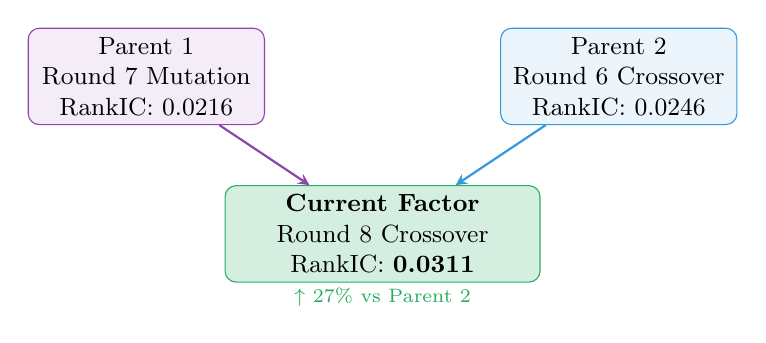
\begin{tikzpicture}[
    node distance=2cm,
    roundbox/.style={rectangle, rounded corners, draw=headerblue, fill=headerblue!10, minimum width=3cm, minimum height=1cm, align=center, font=\small},
    arrow/.style={->, thick, >=stealth}
]
    % Parent nodes
    \node[roundbox, fill=mutationpurple!10, draw=mutationpurple] (p1) at (-3, 2) {Parent 1\\Round 7 Mutation\\RankIC: 0.0216};
    \node[roundbox, fill=crossoverblue!10, draw=crossoverblue] (p2) at (3, 2) {Parent 2\\Round 6 Crossover\\RankIC: 0.0246};
    
    % Current node
    \node[roundbox, fill=metricgreen!20, draw=metricgreen, minimum width=4cm] (current) at (0, 0) {\textbf{Current Factor}\\Round 8 Crossover\\RankIC: \textbf{0.0311}};
    
    % Arrows
    \draw[arrow, mutationpurple] (p1) -- (current);
    \draw[arrow, crossoverblue] (p2) -- (current);
    
    % Label
    \node[font=\scriptsize\color{metricgreen}] at (0, -0.8) {$\uparrow$ 27\% vs Parent 2};
\end{tikzpicture}
\end{center}

\end{evolutionbox}

%%%%%%%%%%%%%%%%%%%%%%%%%%%%%%%%%%%%%%%%%%%%%%%%%%%%%%%%%%%%%%%%%%%%%%%
% Hypothesis
%%%%%%%%%%%%%%%%%%%%%%%%%%%%%%%%%%%%%%%%%%%%%%%%%%%%%%%%%%%%%%%%%%%%%%%
\begin{hypothesisbox}

\textbf{Core Hypothesis:}\\
A regime-aware dual-source momentum factor that combines institutional-driven structural momentum (validated by healthy microstructure) and retail-driven speculative momentum (characterized by high attention and deteriorating fundamentals), dynamically weighted by market volatility: amplifying institutional signals in stable regimes and retail reversal signals in turbulent regimes, will generate superior predictive returns.

\vspace{0.3cm}

\begin{tabular}{@{}p{0.3\textwidth}p{0.65\textwidth}@{}}
\toprule
\textbf{Component} & \textbf{Description} \\
\midrule
\textbf{Concise Observation} & Parent strategies separately targeting institutional trends and retail herding show moderate predictive power (RankIC $\sim$0.02-0.025), suggesting combined signals could capture complementary market dynamics. \\
\midrule
\textbf{Concise Justification} & Sustainable price trends require institutional sponsorship and orderly trading, while retail-driven bubbles lack fundamental support and reverse under stress; a hybrid model exploiting both can enhance robustness across market regimes. \\
\midrule
\textbf{Concise Knowledge} & If institutional accumulation coincides with strong price-volume correlation and low volatility, it indicates sustainable momentum; when retail herding in high-attention stocks occurs alongside declining institutional ownership and high volatility, it signals fragile momentum prone to reversal. \\
\bottomrule
\end{tabular}

\end{hypothesisbox}

%%%%%%%%%%%%%%%%%%%%%%%%%%%%%%%%%%%%%%%%%%%%%%%%%%%%%%%%%%%%%%%%%%%%%%%
% Backtest Metrics
%%%%%%%%%%%%%%%%%%%%%%%%%%%%%%%%%%%%%%%%%%%%%%%%%%%%%%%%%%%%%%%%%%%%%%%
\begin{metricsbox}

\begin{center}
\begin{tabular}{@{}lccc@{}}
\toprule
\textbf{Metric} & \textbf{Current Factor} & \textbf{SOTA Baseline} & \textbf{Comparison} \\
\midrule
\textbf{IC} & 0.0126 & 0.0058 & \textcolor{metricgreen}{$\uparrow$ 117\%} \\
\textbf{ICIR} & 0.0781 & -- & -- \\
\textbf{Rank IC} & \textbf{0.0311} & 0.0220 & \textcolor{metricgreen}{$\uparrow$ 41\%} \\
\textbf{Rank ICIR} & 0.1932 & -- & -- \\
\midrule
\textbf{Annualized Return} & 7.80\% & 5.2\% & \textcolor{metricgreen}{$\uparrow$ 50\%} \\
\textbf{Information Ratio} & 0.963 & 0.973 & \textcolor{alertred}{$\downarrow$ 1\%} \\
\textbf{Max Drawdown} & -11.37\% & -7.3\% & \textcolor{alertred}{$\downarrow$ 56\%} \\
\bottomrule
\end{tabular}
\end{center}

\vspace{0.3cm}

\textbf{Detailed Backtest Results:}
\begin{center}
\small
\begin{tabular}{@{}ll|ll@{}}
\toprule
\textbf{Metric} & \textbf{Value} & \textbf{Metric} & \textbf{Value} \\
\midrule
Daily Excess Return (w/o cost) & 0.0328\% & Daily Excess Return (w/ cost) & 0.0128\% \\
Excess Return Std & 0.52\% & Turnover (FFR) & 100\% \\
L2 Train Loss & 0.9936 & L2 Valid Loss & 0.9962 \\
\bottomrule
\end{tabular}
\end{center}

\end{metricsbox}

%%%%%%%%%%%%%%%%%%%%%%%%%%%%%%%%%%%%%%%%%%%%%%%%%%%%%%%%%%%%%%%%%%%%%%%
% Feedback & Evaluation
%%%%%%%%%%%%%%%%%%%%%%%%%%%%%%%%%%%%%%%%%%%%%%%%%%%%%%%%%%%%%%%%%%%%%%%
\begin{feedbackbox}

\textbf{\faSearch\ Observations:}\\
The current experiment tested two components of the proposed regime-aware dual-source momentum hypothesis: \texttt{Institutional\_Momentum\_Score\_20D} and \texttt{Retail\_Herding\_Divergence\_10D}. Results show mixed performance compared to SOTA:
\begin{itemize}
    \item \textcolor{metricgreen}{\faCheckCircle} Higher annualized return (0.078 vs 0.052)
    \item \textcolor{metricgreen}{\faCheckCircle} Higher IC (0.013 vs 0.006), indicating stronger predictive power
    \item \textcolor{alertred}{\faTimesCircle} Larger max drawdown (-0.114 vs -0.073)
    \item \textcolor{alertred}{\faTimesCircle} Slightly lower information ratio (0.963 vs 0.973)
\end{itemize}

\vspace{0.3cm}

\textbf{\faBalanceScale\ Hypothesis Evaluation:}\\
Results partially support the hypothesis. Improved annualized return and IC suggest that combining institutional and retail momentum signals has merit. However, deterioration in risk metrics (higher drawdown, lower information ratio) indicates that without proper regime-adaptive weighting, the combined signals may amplify risks during turbulent periods. The hypothesis likely requires all three components (institutional momentum, retail herding, volatility-adaptive weighting) to work effectively together.

\vspace{0.3cm}

\textbf{\faFlag\ Decision:} \colorbox{alertred!20}{\textcolor{alertred}{\textbf{REJECTED}}} (decision: false)

\textbf{\faExclamationTriangle\ Reason:}\\
The current factor shows potential but has complexity issues that may lead to overfitting. A simpler approach should:
\begin{enumerate}
    \item Use 20-day price-volume correlation as institutional momentum
    \item Use 5-day average intraday returns as retail attention proxy
    \item Weight these signals by a simple volatility regime indicator (e.g., ratio of recent to historical volatility)
\end{enumerate}
This maintains the core dual-source concept but significantly reduces complexity. The simplified formulation should improve generalization while capturing the hypothesized regime-dependent behavior.

\end{feedbackbox}

%%%%%%%%%%%%%%%%%%%%%%%%%%%%%%%%%%%%%%%%%%%%%%%%%%%%%%%%%%%%%%%%%%%%%%%
% Cache Information
%%%%%%%%%%%%%%%%%%%%%%%%%%%%%%%%%%%%%%%%%%%%%%%%%%%%%%%%%%%%%%%%%%%%%%%
\begin{tcolorbox}[colback=gray!5, colframe=darkgray, fonttitle=\bfseries, title={\faDatabase\ Data Cache Location}, arc=2mm, boxrule=0.5pt]
\small
\begin{tabular}{@{}ll@{}}
\textbf{Workspace Path:} & \texttt{/mnt/DATA/quantagent/AlphaAgent/RD-Agent\_workspace\_exp\_20260122\_002359} \\
\textbf{Factor Directory:} & \texttt{41e5297ea03142ef9b48c07e517fac01} \\
\textbf{Result File:} & \texttt{result.h5} \\
\textbf{Pickle Cache:} & \texttt{/mnt/DATA/quantagent/AlphaAgent/pickle\_cache\_exp\_20260122\_002359} \\
\end{tabular}
\end{tcolorbox}

%%%%%%%%%%%%%%%%%%%%%%%%%%%%%%%%%%%%%%%%%%%%%%%%%%%%%%%%%%%%%%%%%%%%%%%
% Footer
%%%%%%%%%%%%%%%%%%%%%%%%%%%%%%%%%%%%%%%%%%%%%%%%%%%%%%%%%%%%%%%%%%%%%%%
\vfill
\begin{center}
\rule{\textwidth}{0.5pt}\\[0.2cm]
{\small\color{darkgray} This card is auto-generated by AlphaAgent Factor Mining System | Data Source: trajectory\_pool.json \& all\_factors\_library.json}\\
{\footnotesize\color{gray} Generated: \today}
\end{center}

\end{document}
